\chapter{Problem analysis}\label{cha:problem-analysis}
A digital image consists of pixels. In a grayscale image, each pixel has a value between 0 and 255, where 0 is black and 255 is white. In a color image each pixel has three such values - one for each color red, green, and blue. The number of pixels in an image is the number of pixels in the image multiplied by the number of colors. For example, a 28x28 grayscale image has 784 pixels, while a 28x28 color image has 2352 pixels.

In this way each pixel represents a feature (dimension) of the image. As the size of images increase this quickly becomes a large number of features, and for the purpose of \gls{ml} it is likely not necessary to use all of them. The process of choosing the most important features is called feature selection, and leads to dimensionality reduction, the topic of this report.


\section{Dimensionality reduction}\label{sec:dimensionality-reduction}
In general, dimensionality reduction transforms data with many features (dimensions) into a new representation of the data with fewer features while preserving as much relevant information as possible. Dimensionality reduction is made by finding a transformation of the data that maps the data to some lower dimensional space while keeping the mean distances between the data points~\cite{dimensionality-reduction-comparative-review}.

Dimensionality reduction can be divided into two categories: linear and nonlinear methods, described in Section \ref{sec:linear-vs-nonlinear}. This section presents some of the standard methods from both categories.

\todo[inline]{Linear methods are based on the assumption that the data is linear. 
A linear dataset is one in which all possible prediction outcomes can be obtained by combinations of the original features without any additional interactions. 
You can show an example of linear data for regression and classification. 
Note that this difference is not so strict as some methods could be thought of as both}


\subsection{Linear methods}\label{subsec:linear-methods}
The linear methods covered are: \gls{pca}, \gls{fa}, \gls{nmf}, and \gls{lda}.


\subsubsection{Principal Components Analysis}\label{subsubsec:principal-components-analysis}
\gls{pca} is a linear method used to reduce a dataset's dimensionality by projecting it onto a lower dimensional subspace, retaining as much of the variance as possible. The best projection is found through the directions of maximum variance in the data based on the covariance matrix and then projecting the data onto those directions. The directions of maximum variance are principal components, and the projection results from the \gls{pca}~\cite{dimensionality-reduction-comparative-review}.


\subsubsection{Factor Analysis}\label{subsubsec:factor-analysis}
\gls{fa} is very similar to \gls{pca}, and \gls{pca} may be called a type of \gls{fa}. However, \gls{fa} is based on the assumption that the data is generated by a linear combination of a few latent variables called factors and that the observed variables are a linear combination of the latent variables plus some noise.

The goal of \gls{fa} is to find the factors that explain the most covariance in the data. Intuitively, related items have stronger mathematical correlations and can thus be grouped with less loss of information. Once the correlations are determined, a rotation is performed to make the factors easier to interpret~\gls{fa}~\cite{decoster-1998-factor-analysis-overview}.


\subsubsection{Non-negative matrix factorization}\label{subsubsec:non-negative-matrix-factorization}
\gls{nmf} constructs approximate factorizations of a non-negative data matrix $V$ into two non-negative matrices $W$ and $H$ such that $V \approx WH$. The non-negativity constraints permit the intuition that data may represent parts forming a whole, which can be thought of as a sum of parts~\cite{lee-1999-learning-nmf}. For example, a text document may represent a combination of topics, and each may represent a combination of words.


\subsubsection{Linear Discriminant Analysis}\label{subsubsec:linear-discriminant-analysis}

\gls{lda} is quite similar to \gls{pca} since they both try to project data into a hyperplane. Still, instead, \gls{lda} tries to maximize class separability, making it easier to contrast classes. \gls{lda} finds the hyperplane with the most separation between the classes and keeps the data points with the same class as close together as possible. This is a three-step process. The first step is to determine the separation between different classes (between-class variance) as the distance between the means of each class. Secondly, the distance between the mean and samples of each class (within-class variance) is calculated. The third step is creating a lower dimensional representation that maximizes the between-class variance and minimizes the within-class variance~\cite{linear-discriminant-analysis-tutorial}.


\subsection{Non-linear methods}\label{subsec:non-linear-methods}
Sometimes high-dimensional data may contain non-linear relationships, which linear methods cannot capture. It has been shown that \gls{pca} fails to find significant components in the swiss-roll dataset~\cite{tennenbaum}. In such cases, non-linear methods are used. The non-linear methods covered are \gls{kpca}, \gls{mds}, and \gls{isomap}.


\subsubsection{Kernel Principal Component Analysis}\label{subsubsec:kernel-principal-component-analysis}
\gls{kpca} is an extension of \gls{pca}, and it projects the data onto a higher dimensional plane, where \gls{pca} is performed. 
The first step is to construct the kernel matrix from the data. The kernel matrix is a matrix of the dot products of the data points, the kernel matrix is used like the covariance matrix in \gls{pca}~\cite{kernel-pca}. In the kernel matrix the data is in a higher dimensional space, where the data is linear separable. By using the kernel function, \gls{kpca} exposes the kernel trick, which is instead of calculating the dat into a higher dimensional space, it calculates the inner product between the datapoints, which is computationally cheap to calculate instead of calculating every datapoint into a higher dimensional space.
The kernel matrix is then centered by subtracting the mean of each row and column. This matrix is also called the Gram matrix. The Gram matrix is then used to find eigenvectors and eigenvalues. By using the kernel trick, \gls{kpca} can compute eigenvalue decomposition, as in \gls{pca}.The eigenvectors are then used to project the data onto a higher dimensional space, where \gls{pca} is performed. The eigenvectors with the highest eigenvalues are the principal components, and the projection is the data projected onto the principal components~\cite{kernel-pca}. 

\subsubsection{Isometric Feature Mapping}\label{subsubsec:isometric-feature-mapping}
\gls{isomap} is another non-linear method that is a special case of \gls{cmds}. It is assumed that \gls{isomap} is suited to discover manifolds of arbitrary dimensionality and that it guarantees an approximation of the true structure of the manifold~\cite{tennenbaum}.

The first step in \gls{isomap} is to map the data points in a graph. The graph is constructed by connecting each point to its nearest neighbors. The user sets the number of nearest neighbors. The nearest neighbors are found by using the Euclidean distance. The Euclidean distance is the linear distance between two points in a Euclidean space~\cite{Multidimensional-Scaling-Sammon-Mapping-and-Isomap}.

In the second step, \gls{isomap} finds the Geodesic distance between each point~\cite{Multidimensional-Scaling-Sammon-Mapping-and-Isomap}. The Geodesic distance is the shortest distance between two points on the surface of a sphere. The Geodesic distance is calculated by finding the shortest path between two points on a graph. The graph is constructed by connecting each point to its nearest neighbors. The shortest path can be found by using the Dijkstra algorithm~\cite{multi-dimensional-scaling-leeuw}.

The final step in \gls{isomap} is finding the data's \gls{mds} projection. The \gls{mds} projection is found by minimizing the stress function. The stress function is the sum of the squared differences between the distances in the original data and the distances in the projected data~\cite{multi-dimensional-scaling-leeuw}, so the stress function finds the slightest change in the data. The minimum of this stress function will be the best reproduction of the data in lower dimensional space according to the \gls{isomap} algorithm. 



\subsection{Choice of dimensionality reduction}
Four different dimensionality reduction methods have been chosen to be in the implementation. These are linear and nonlinear methods, particularly \gls{pca}, \gls{lda}, \gls{kpca}, and \gls{isomap}. The group chose these four because they cover the spectrum of options well and are some of the most used. Only four were selected to keep the project's focus tight and the right amount of depth versus breadth of the project.

%ISOMAP 


%The geodesic distance is used in \gls{isomap} to find the shortest distance between two points in a dataset. %These will be clarified first before clarifying \gls{isomap}. 

%\subparagraph{Multi Dimensional Scaling}\label{subsec:multi-dimensional-scaling}
%\gls{mds} is a non-linear method that is used to reduce the dimensionality of a dataset by projecting it onto a lower dimensional subspace, while preserving as much of the variance between the data as possible. The projection is found by calculating the best result from the \gls{mds} function which is a modified version of the STRESS function. The STRESS function finds the least change in data when in the case of \gls{mds} is when reducing the dimensionality~\cite{multi-dimensional-scaling-leeuw}.

%\subparagraph{Geodesic distance}\label{subsec:geodesic-distance}
%Geodesic is a distance between two points on a surface of a sphere. The geodesic distance between two points is the shortest distance between the two points on the surface of a sphere. The geodesic distance is calculated by finding the shortest path between two points on a graph. The graph is constructed by connecting each point to its nearest neighbors. The shortest path is found by using the Dijkstra's algorithm~\cite{multi-dimensional-scaling-leeuw}.


% In this project we will focus on dimensionality reduction for the purpose of computer vision, and in particular for the MNIST dataset.


% In this project we will study some common methods of dimensionality reduction using the MNIST dataset for digit recognition.
\newacronym{relu}{ReLU}{Rectified Linear Unit}

\section{Machine Learning}\label{sec:machine-learning}
To determine the relevant dimensionality reduction methods to compare for the project, it is necessary to understand the basics of machine learning. This section describes the basics of machine learning and the different types of machine learning problems.


\subsection{Machine learning pipeline}\label{subsec:machine-learning-pipeline}
Figure~\ref{fig:basic-machine-learning-pipeline} shows the simplified and generalized steps in the pipeline of a machine learning model. The machine learning pipeline is divided into four main steps: data collection, feature engineering, model training and model evaluation.


\begin{figure}[htb!]
    \centering
    \begin{tikzpicture}
        \node (b) [state] {feature engineering};
        \node (c) [state, shift={($(b.east)+(2cm,0)$)}] {model};
        \node (a) [state, shift={($(b.west)+(-2cm,0)$)}] {data};
        \node (d) [state, shift={($(c.east)+(2cm,0)$)}] {evaluation};
        \node (e) [state, shift={($(b.south)+(0,-2cm)$)}] {parameters};

        \draw[arrow, ->] (a) -- node[above,scale=.70,align=center,] {} (b);
        \draw[arrow, ->] (b) -- node[above,scale=.70,align=center,] {} (c);
        \draw[arrow, ->] (c) -- node[above,scale=.70,align=center,] {} (d);
        \draw[arrow, ->] (e) -- node[above,scale=.70,align=center,] {} (c);

        \draw[arrow, ->] (d.north) -- ++(0,0.75) -| (b);
        \draw[arrow, ->] (d.south) -- ++(0,-0.75) -| (c);
    \end{tikzpicture}
    \caption{Simplified machine learning pipeline}
    \label{fig:basic-machine-learning-pipeline}
\end{figure}


The box with the name data represents the input to the machine learning pipeline. The data can be in different formats, such as images, text, audio, video, etc. The data is usually stored in a database or in a file. This is also the step where the data is cleaned and preprocessed.

Feature engineering represents the step where the data is transformed through dimensionality reduction. The reduced data is the input to the machine learning model.

Model training is the process of training the model with the data. This is done by splitting the data into a training set and a validation set. The training set is used to train the model to predict the output with highest possible accuracy. The validation set is used to evaluate the model, and may use cross validation to get a more accurate evaluation that avoids overfitting. The model depends on the type of machine learning problem.

Model evaluation represents the step where the model is evaluated. The evaluation is done by comparing the predictions of the model with the actual values. The evaluation is done on the validation set. The evaluation is done by using metrics such as accuracy, precision, recall, F1 score, etc. The evaluation is done to determine the performance of the model and to determine if the model is overfitting or underfitting.

The box with the name "parameters" represents the hyperparameters of the machine learning model. These parameters are set before training the model. The hyperparameters are usually set by the user, but can also be set by the machine learning model itself. The hyperparameters are usually set by trial and error, but there are also methods to find the best hyperparameters.

The arrows represent how machine learning models continously learn. The model is trained on the training set, and then evaluated on the validation set. The model is then updated with the new information, and the process is repeated. This is called the training loop. The training loop is repeated until the model converges, or until the model is no longer improving. The model is then evaluated on the test set, and the evaluation is used to determine the performance of the model.


\subsection{Data}\label{subsec:data}
Because the machine learning pipeline starts with the data, the choice of dataset for the project will impact all the following steps in the pipeline.

Most importantly the data must allow for the evaluation of the dimensionality reduction methods. Therefore, the dataset should be large enough dimensionally to perform meaningful dimensionality reduction. Furthermore, a well researched dataset is preferred, as it is more likely to be well suited for the evaluation of dimensionality reduction methods.

Based on the above requirements the \gls{mnist}~\cite{lecun-mnist-database} dataset is chosen. It is a dataset of images of 28x28 grayscale images of handwritten digits, making it well suited for the evaluation of dimensionality reduction methods, as the images are large enough to perform meaningful dimensionality reduction. Furthermore, the dataset is well researched, and has been used in many papers~\cite{lecun-mnist-database}.

In fact \gls{mnist} is so well researched that it may be considered overused~\cite{fashion-mnist}. If time permits, two similar datasets may be used in the project. The first is the \gls{fashion-mnist}~\cite{fashion-mnist} dataset, which is a variant of \gls{mnist} with images of clothing instead of handwritten digits. The second is the \gls{cifar}~\cite{krizhevsky-cifar} dataset, which consists of 50,000 training images and 10,000 test images of 32x32 color images of 10 different classes of objects.


\subsection{Feature engineering}\label{subsec:feature-engineering}
The theory deciding the choice of dimensionality reduction methods is described in Chapter~\ref{cha:theory}.

\todo[inline]{Some notes: normal distribution is relevant for LDA in particular apparently \url{https://www.rikvoorhaar.com/normal-data/}. FA is unlikely to be practical. PCA is the most common method}

\subsection{Machine learning models}\label{subsec:machine-learning-models}
Because \gls{mnist} is a set of labeled images, the machine learning problem is a multi-class classification supervised learning problem within the domain of computer vision, with the goal to train a model to predict the correct digit represented in an image.

Several machine learning models are used for image classification in general, and \gls{mnist} in particular~\cite{lecun-mnist-database,IBM-computer-vision,convolutional-neural-networks-convnets,multi-column-neural-network-ciregan}.

This project is not particularly concerned with the choice of machine learning model, but rather with the choice of dimensionality reduction methods. Therefore, \gls{svm} is chosen as the machine learning model. It is a relatively understandable model as it has similarities to the \gls{lda} method for dimensionality reduction \todo{perhaps better not to write this}, and has already been used with \gls{mnist} without dimensionality reduction~\cite{lecun-mnist-database}.

%why is there are the quora link.
% https://www.quora.com/What-is-the-difference-between-SVM-and-linear-discriminant-analysis

Additionally, a \gls{cnn} is used to compare the results of the dimensionality reduction methods with a more complex model. It is also used to compare the performance of the dimensionality reduction methods with a model that is not based on linear algebra. We will present what multi-class classification is, then explain how \gls{svm} and \gls{cnn} work.


\subsubsection{Multi-class classification}\label{subsubsec:multi-class-classification}
The \gls{mnist} dataset presents a multi-class classification problem, as the images can represent any of the 10 digits. The \gls{svm} model however is a binary classification model, and thus has to be adapted to the multi-class classification problem. There are two approaches to this problem: \gls{ovo} and \gls{ova}.

\gls{ovo} is a method where the model is trained on all possible combinations of two classes. For example, if there are 5 classes, the model is trained on 10 different models, one for each combination of two classes, this makes it computationally expensive as it has to go througth every combination. The model is then evaluated on all the models, and the class with the highest score is chosen as the predicted class.

\gls{ova} however is a method where the model is trained faster than in \gls{ovo}, as it only uses one class to distinguish if the data is similar or not. For example, if there are 5 classes, the model is trained on 5 different variations of the model, one for each class. This makes \gls{ova} good to distinguish between the current class that is being modeled from the other classes, however in \gls{ova} it is harder to distinguish between the other classes that is not being trained on. The model is then evaluated on all the models, and the class with the highest score is chosen as the predicted class~\cite{james-statistical-learning}.

\gls{ovo} is more computationally expensive than \gls{ova}, but is more accurate. The choice of \gls{ovo} or \gls{ova} is therefore a trade-off between accuracy and computational cost~\cite{james-statistical-learning}. The \gls{svm} model is chosen because it is a relatively simple model, and thus \gls{ova} is chosen as it is faster than \gls{ovo}.


\subsubsection{Support Vector Machine}\label{subsubsec:support-vector-machine}
\gls{svm} is a supervised learning model that classifies data by finding a mapping (hyperplane) that separates the classes in data~\cite{faster-svm}. \gls{svm} is also known as a large-margin classifier, which means that it relies on finding \textcquote{faster-svm}{a maximum-margin hyperplane to separate classes}. \gls{svm}, as the name implies, uses support vectors, are the 'vectors' that are closest to the function defining the mapping, and alterations on those data points will influence the hyperplane. For our purposes \gls{svm} is a promising model, since it is capable of defining a decision boundry which separates the classes the most. Such approach may be similar to how \gls{lda} works. An interesting property of \gls{svm} is that it can have among other parameters a kernel function, which can be tuned whether the data is linearly separable or not~\cite{faster-svm}. The kernel function that \gls{svm} shares resemblance to the way \gls{kpca} works, as it also uses a kernel function.


\subsubsection{Convolutional Neural Networks}\label{subsubsec:convolutional-neural-networks}
We assume that the reader is familiar with \gls{nn}s. The \gls{cnn}s are a specialized form of \gls{nn} that are mostly used for pattern recognition in images~\cite{introduction-to-cnn}. The reason we chose to work with \gls{cnn} is because, while normal \gls{nn}s are able to solve the classification problem regarding \gls{mnist}, they might not be as powerful as \gls{cnn}. The robustness of the \gls{cnn} can be shown in the sources~\cite{lecun-mnist-database, mnist-classification-benchmark}, where \gls{cnn}s are depicted as being 'state-of-the-art' machine learning models based on the minimum error rate that they achieve.


In our project it might not make a major difference, but using a \gls{cnn} can be better suited for image classifcation, as presented. Furthermore, according to Keiron et al.\ ~\cite{introduction-to-cnn}, \gls{nn}s are more prone to overfitting due to the layers being fully-connected, which increases the number of parameters, thereby increasing the complexity of the model. Another reason is the practicality / scalability of the model, as Keiron highlighted in his report, where he depicted a possible issue with \gls{nn}. The \gls{mnist} consists of $28 \times 28$ \textit{monochrome} pixels, which is relatively simple, compared to the real-world images which can be bigger, and have three colors / channels. We know that \gls{nn}s are fully-connected layers, in essence, neurons are connected to all the neurons in the previous layer, and Figure \ref{fig:nn-example-architecture} can provide a visual aid. When the amount of pixels is large, and colorized, then so should the size of the \gls{nn} be~\cite{introduction-to-cnn}.

\begin{figure}[htb!]
    \centering
    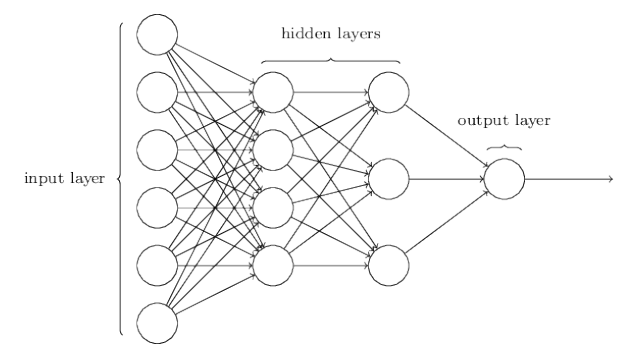
\includegraphics[width=0.65\textwidth]{figures/michael-nielsen-nn-architecture.png}
    \caption{An example of a neural network architecture~\cite{michael-nielsen-nn}}
    \label{fig:nn-example-architecture}
\end{figure}

The difference between \gls{nn} and \gls{cnn} is the among others the architectural blueprint. In \gls{cnn} neurons also have another property: the neurons are arranged in three dimensions: \textcquote{introduction-to-cnn}{the spatial dimensionality of the input(\textbf{height} and the \textbf{width}), and the \textbf{depth}}. The spatial dimensionality is the pixels, and the depth is one, since \gls{mnist} is monochrome.


%Ugly figure and not 100% visual, but it is simple
\begin{figure}[htb!]
    \centering
    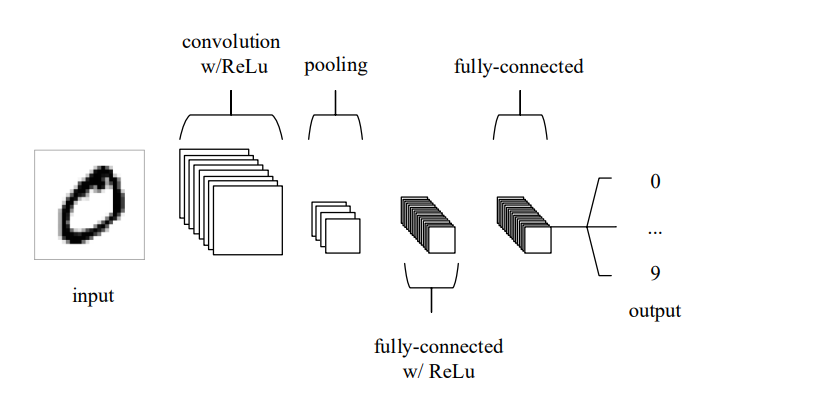
\includegraphics[width=0.8\textwidth]{figures/cnn-simple-architecture.png}
    \caption{An example of a convolutional neural network architecture~\cite{introduction-to-cnn}}
    \label{fig:simple-cnn-architecture}
\end{figure}
%Blog-like structure where CNN is depicted

\gls{cnn}'s architecture constitutes three different types of layers: convolutional layers, pooling layers, and fully-connected layers. The architecture of a \gls{cnn} can be shown in Figure \ref{fig:simple-cnn-architecture}. The convolutional layers \textcquote{introduction-to-cnn}{will determine the output of neurons of which are connected to local regions of the input}, which is also called a convolution. The pooling layers reduce the number of parameters in the previous layers. The fully-connected layers act as normal \gls{nn} layers~\cite{introduction-to-cnn}.


A convolution, as described, acts as a filter which maps the input to an output matrix $conv$ of size $n \times n$. The mapping is done by the elementwise-multiplication of the input matrix with the $conv$ matrix. The operation can be seen in Figure \ref{fig:convolution}. The manner in which such mapping is achieved is by sliding over the input matrix, from left to right, top to bottom, with a $n \times n$ matrix one pixel at a time. For each convolution operation \gls{relu} is applied to the operation, where \gls{relu} is a function which takes the maximum value between 0 and the input~\cite{google-cnn}.

\begin{figure}[htb!]
    \centering
    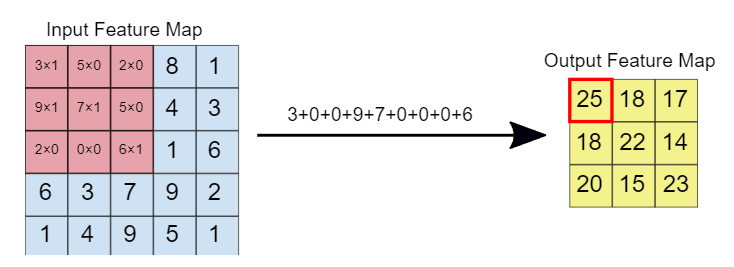
\includegraphics[width=0.7\textwidth]{figures/google-cnn-convolution-example.png}
    \caption{An example of a convolution operation~\cite{google-cnn}}
    \label{fig:convolution}
\end{figure}

In the pooling layer behaves like a convolution, but this time it filters the $conv$ matrix with a $pool$ matrix of size $n \times n$. One method which has been presented~\cite{google-cnn} is the use of max pooling; in the convolutional layer the elementwise multiplication is applied, whereas in max pooling the element with the highest number in the respective matrix is chosen~\cite{google-cnn}. Figure \ref{fig:maxpooling} is provided to show how it works. The pooling layer can be seen as a dimensionality reduction method, because it reduces the data while preserving the original features.

\begin{figure}[htb!]
    \centering
    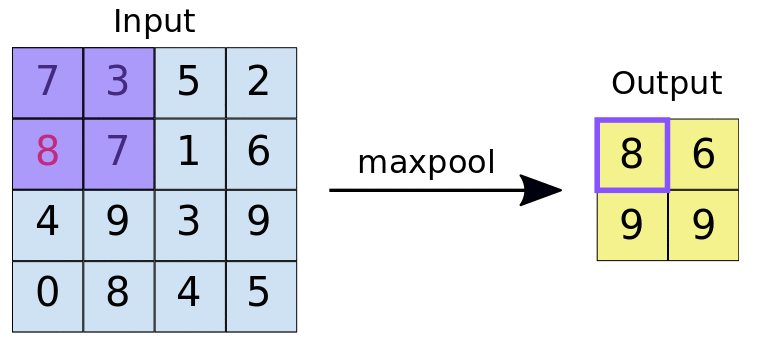
\includegraphics[width=0.5\textwidth]{figures/google-cnn-maxpooling-example.png}
    \caption{An example of a max pooling operation~\cite{google-cnn}}
    \label{fig:maxpooling}
\end{figure}

The last layer is the fully-connected layer, which is connected to all the neurons from the pooling layer. According to Keiron ~\cite{introduction-to-cnn}, the activation function \gls{relu} might be suited to be used in this layer too~\cite{lecun-mnist-database}.

\subsection{Model training}\label{subsec:model-training}
The theory deciding the cross validation methods is described in Chapter~\ref{cha:theory}.



% @book{michael-nielsen-nn,
%   title={Neural networks and deep learning},
%   author={Nielsen, Michael A},
%   volume={25},
%   year={2015},
%   publisher={Determination press San Francisco, CA, USA}
% }
% @misc{faster-svm,
%   doi = {10.48550/ARXIV.1808.06394},
  
%   url = {https://arxiv.org/abs/1808.06394},
  
%   author = {Schlag, Sebastian and Schmitt, Matthias and Schulz, Christian},
  
%   title = {Faster Support Vector Machines},
  
%   publisher = {arXiv},
  
%   year = {2018},
  
%   copyright = {arXiv.org perpetual, non-exclusive license}
% }


% @misc{introduction-to-cnn,
%   doi = {10.48550/ARXIV.1511.08458},
  
%   url = {https://arxiv.org/abs/1511.08458},
  
%   author = {O'Shea, Keiron and Nash, Ryan},
  
%   title = {An Introduction to Convolutional Neural Networks},
  
%   publisher = {arXiv},
  
%   year = {2015},
  
%   copyright = {arXiv.org perpetual, non-exclusive license}
% }


% @misc{mnist-classification-benchmark,
%     url = {https://paperswithcode.com/sota/image-classification-on-mnist},
%     title = {Image Classifcation onf MNIST},
%     year = {2022}
% }

% @misc{google-cnn,
%     organization = {Google},
%     url = {https://developers.google.com/machine-learning/practica/image-classification/convolutional-neural-networks},
%     title = {ML Practicum: Image Classification},
%     year = {2022}
% }



\section{Problem Statement}\label{sec:problem-statement}
\subsection{Audio} 
For models that predict what music is popular or what genre the music is we would like to see how big of an effect feature engineering has for the model. We would like to investigate which kind of dimensionality reduction works best considering both linear and nonlinear aproaches and what they contribute to in the model and when it is a better fit. The performance of these dimensionality reductions is evaluated based on how they affect the performance of the model and their visualisations.

\subsection{Pokemon}
For a model that clasifies Pokemon we would like to see how big of an effect feature engineering has for the model. We would also like to investigate which kind of dimensionality reduction works best and consider both linear and nonlinear aproaches and what they each contribute and when theyre correct to use. The performance of these aproaches might be evaluated based on their visualisations and how they affect model performance.

\subsection{Match data}
For models that predict the outcome of football matches we would like to see how big the effect of feature engineering has for the model. We would also like to investigate which kind of dimensionality reduction works best considering both linear and nonlinear aproaches and what they contribute to in the model and when it is a better fit. The performance of these dimensionality reductions is evaluated based on how they affect the performance of the model and their visualisations.
